\chapter{Habitat of ice reservoirs}

\cleanchapterquote{Ice stupas offer a solution to the shortage of water all our mountain regions are
facing.}{Pema Gyamtsho }{(Director General, International Center for Integrated Mountain Development)}

AIRs cannot be built anywhere. They require favourable weather conditions, sufficient water supply, and specific
topography to amass a seasonal stock of ice. However, these three requirements exhibit drastic
spatio-temporal variations. Therefore, high-resolution datasets are necessary to judge any location's AIR
suitability. 

In this chapter, we base our analysis on the ice stupas built in Swiss and the Indian regions where such
datasets are available. We examine their observed volume variations across different spatial and temporal scales.
Later, we discuss some useful metrics to qualitatively assess the suitability of new construction locations in a
regional and local scale.

\section{Observed ice volume variability}

\subsection{Interregional scale}

\begin{figure}[htb]
\centering
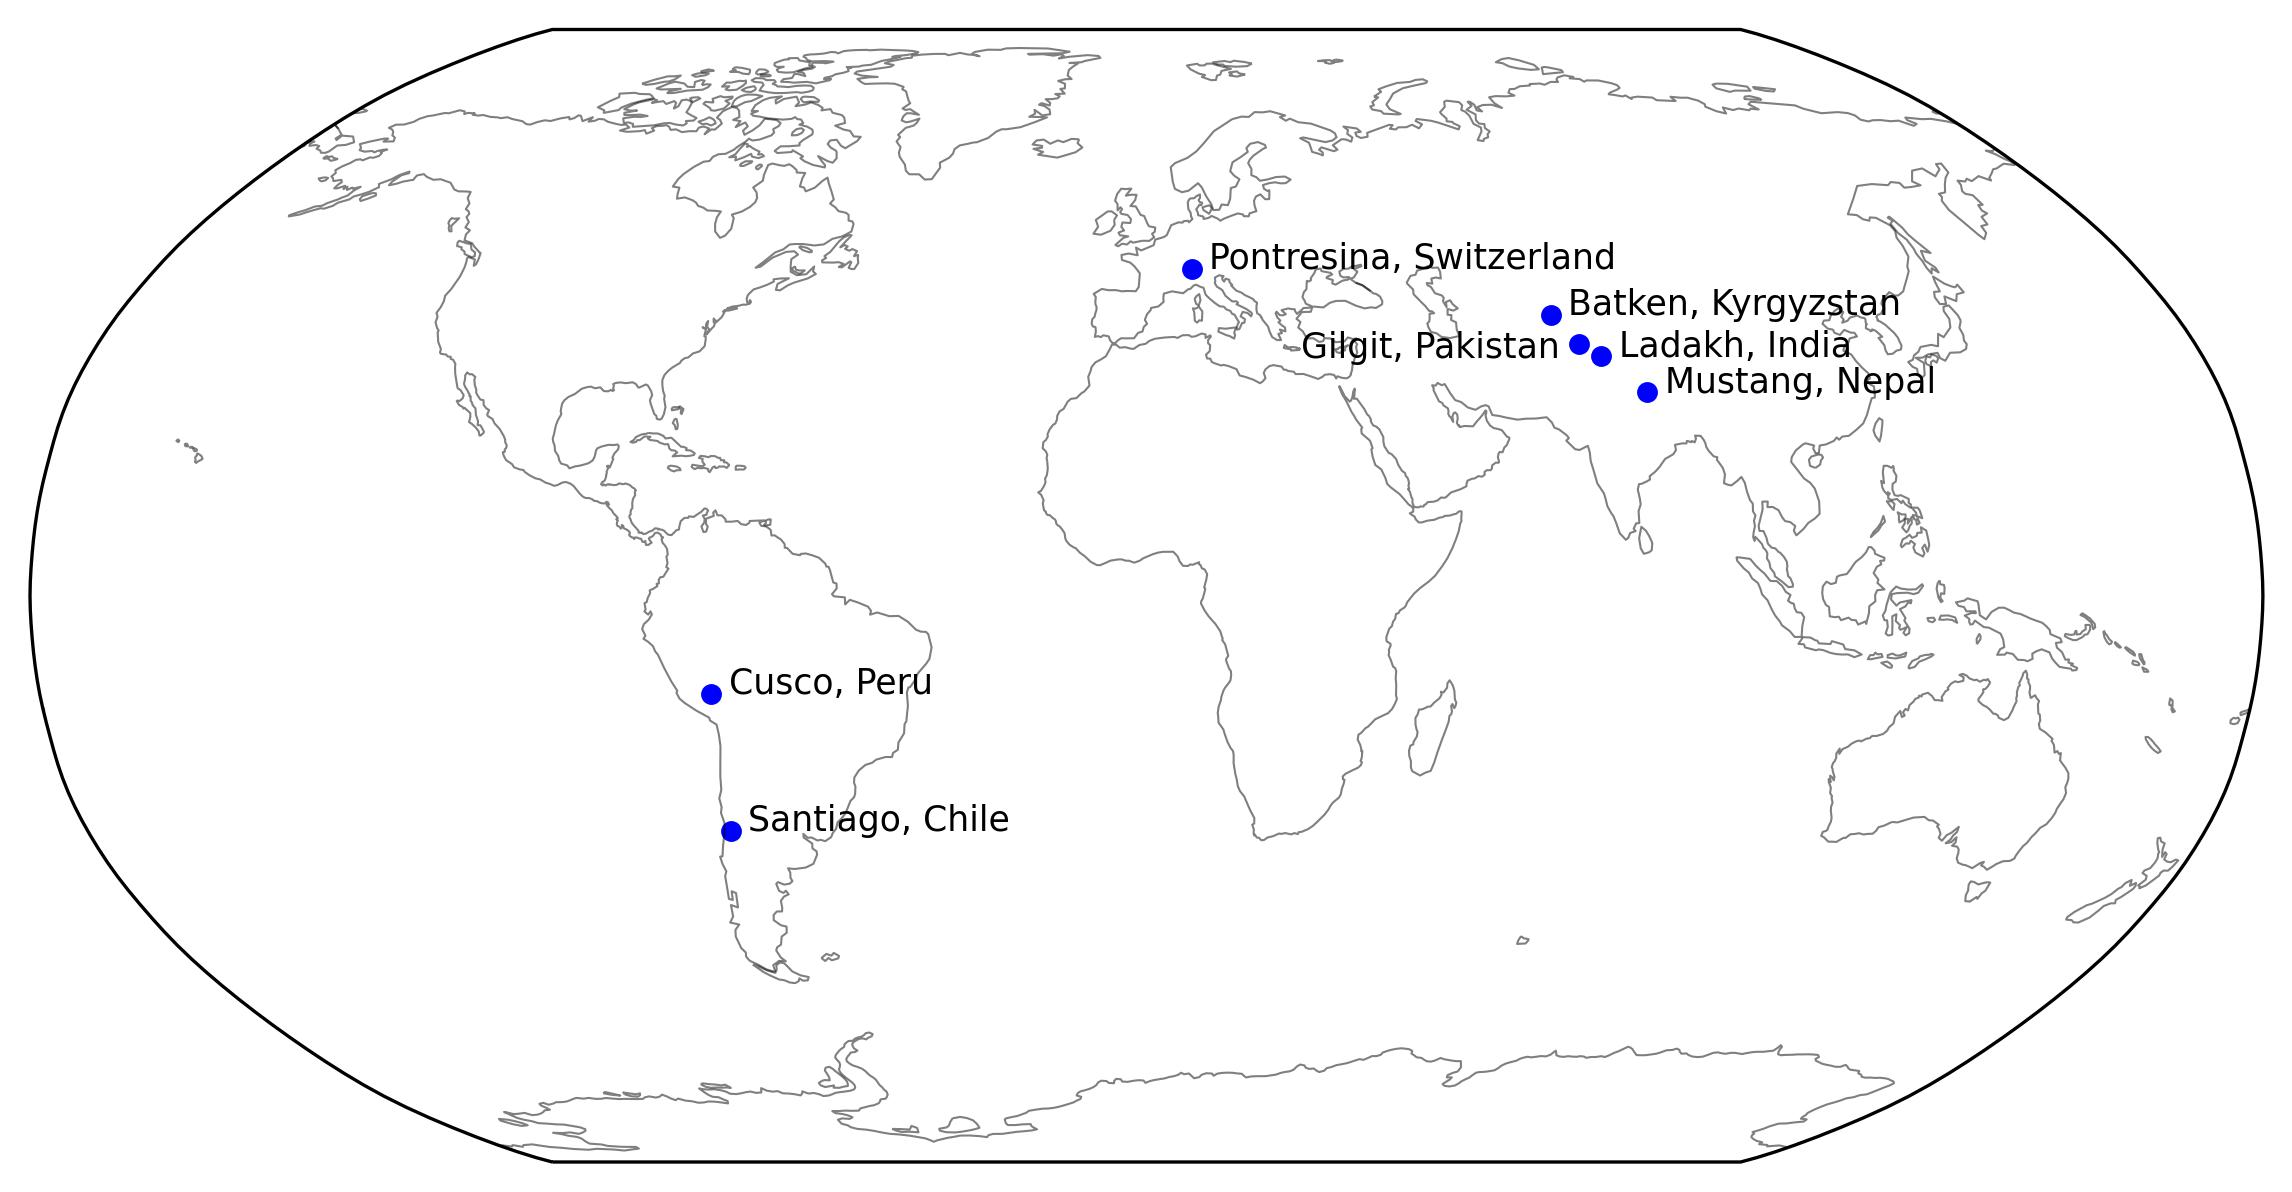
\includegraphics[width=\textwidth]{figs/air_regions.jpg}
\caption{Regions where AIRs have been built.}
\label{fig:AIR_regions}
\end{figure}

AIRs built in the Himalayas, Andes and the Alps show drastic ice volume variations (Fig. \ref{fig:AIR_regions}).
Comparison of ice stupa volume evolution show that the Indian structures grew four times larger than the Swiss ones (Fig.
\ref{fig:2AIRs}). The corresponding freezing rate of the Indian ice stupa was more than ten times higher than
the Swiss one. Sublimation was identified as the driving process of this difference (paper I). These results indicate that the
colder, drier and less cloudy weather characteristics of the Ladakh region made it more suitable to build AIRs
compared to the Guttannen region. 

\subsection{Intraregional scale}

\begin{figure}[htb]
	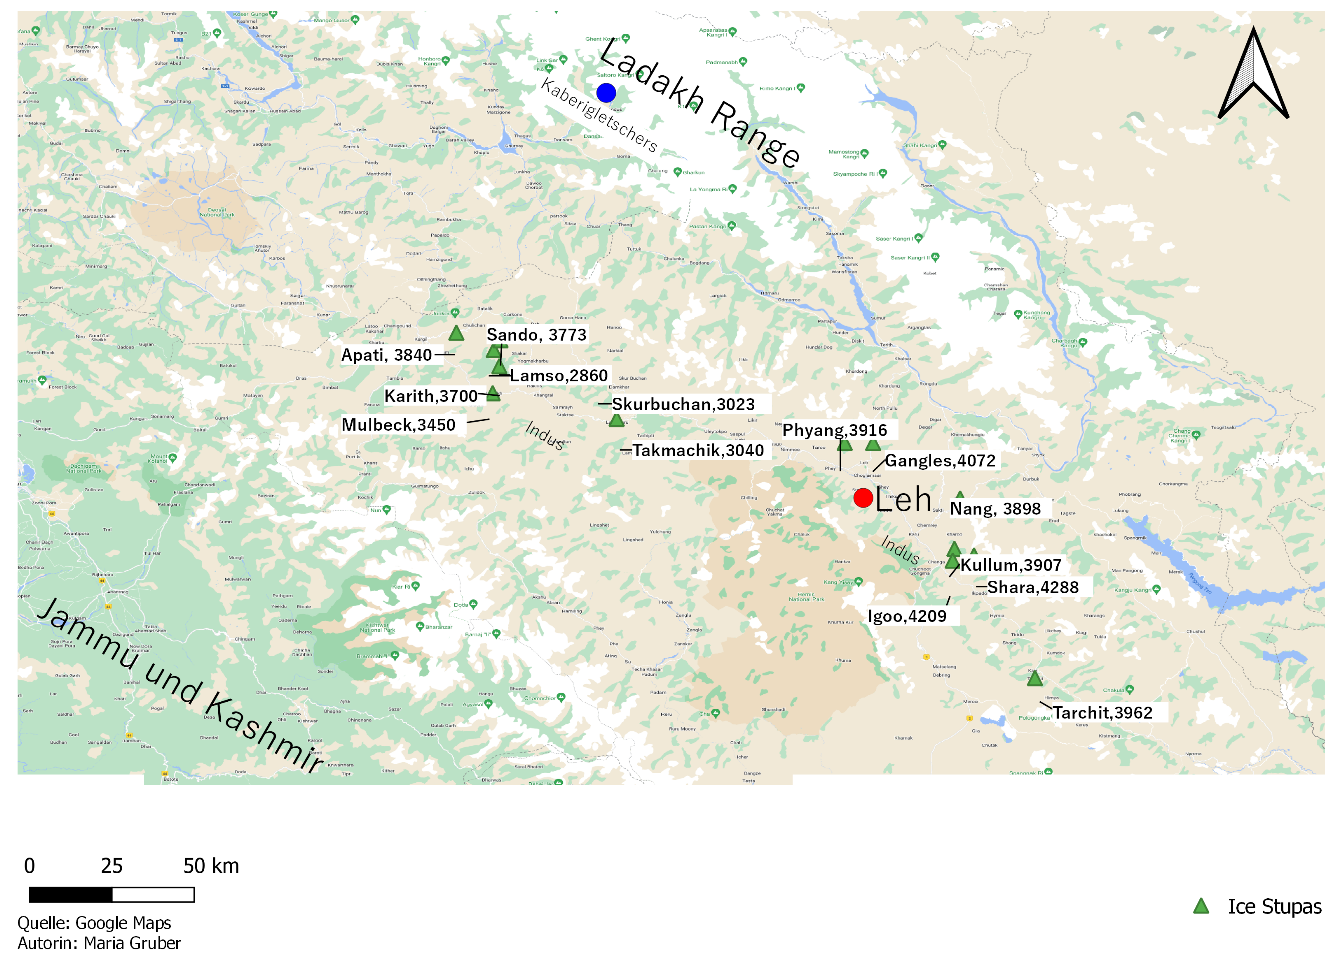
\includegraphics[width=\textwidth]{figs/ISC_villages}
  \caption{Some villages of Ladakh where AIRs have been built. Adapted from \citet{mariagruberIceStupasLadakh2022}.}
	\label{fig:villages}
\end{figure}

We measured ice volumes in more than 14 villages in Ladakh (Fig. \ref{fig:villages}). Their volume variation
reveals a correlation with the altitude of the construction location (Fig. \ref{fig:altvsvol}). This correlation
indicates that elevation gain of 100 $m$ causes a corresponding ice volume gain of 1 million litres. However,
some locations with lower altitude exhibit higher volumes compared to those with a higher altitude. This is due
to topographic effects of shadow valleys that reduce the sunshine hours of the location
\citep{mariagruberIceStupasLadakh2022}.

\begin{figure}[htb]
\centering
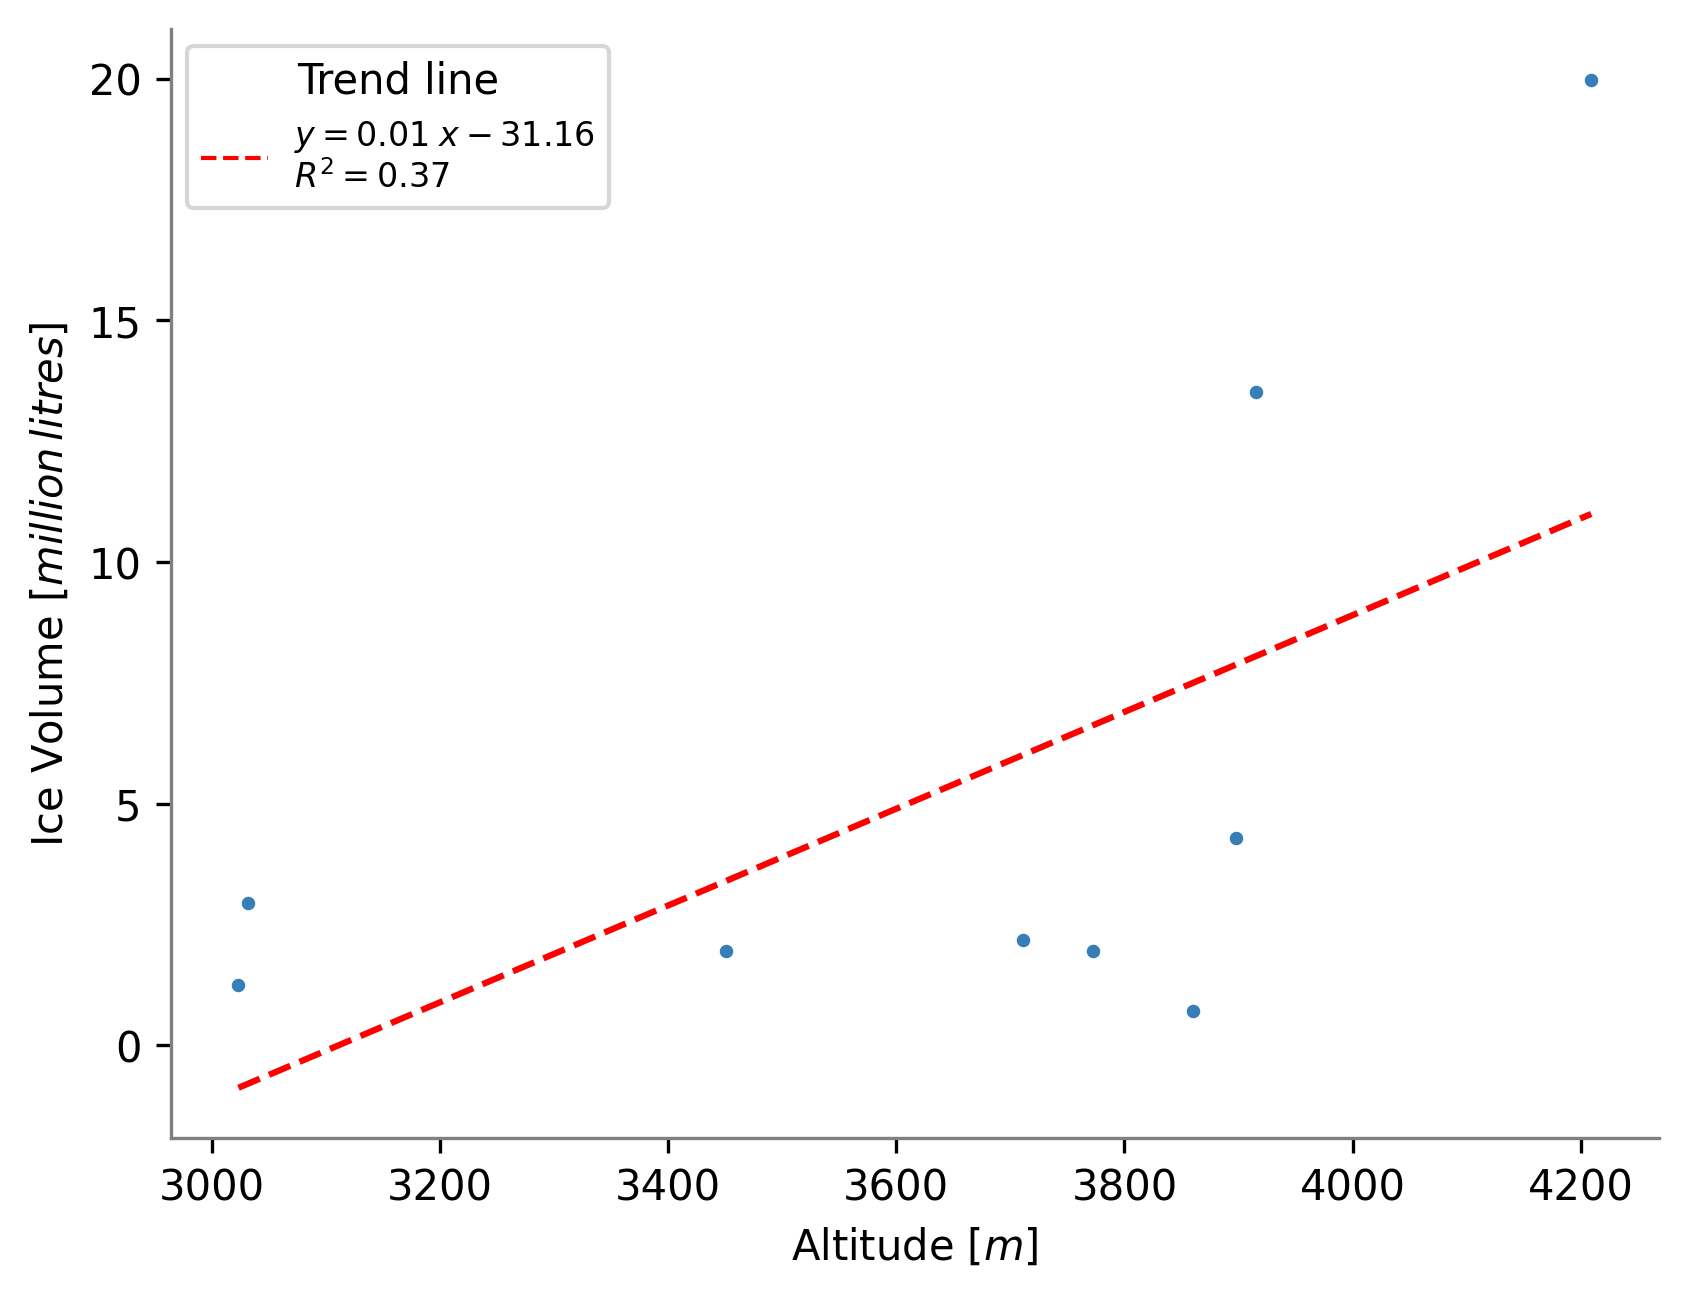
\includegraphics[width=\textwidth]{figs/altitudevsvolume.png}
\caption{Relationship of measured ice volume with altitude of AIRs built during winter of 2019-20 across
different villages in Ladakh. Adapted from \citet{mariagruberIceStupasLadakh2022}.}
\label{fig:altvsvol}
\end{figure}

Some ice stupas built in villages above 4200 m a.s.l. (Shara and Igoo) have also been observed to last beyond a
summer melt season (Fig. \ref{fig:PIR}). However, such favourable weather conditions
remain to be discovered in the Swiss mountains. A possible way to study this question is to decrease the air temperature uniformly
(temperature change $\Delta T$). This will imply a stronger negative sensible heat flux in summer, thus
accelerating ice stupa growth and slowing down its decay. Such simulations were produced in paper III for an ice
stupa grown in the Diavolezza site at an altitude of 2080 m a.s.l. . We found a break-even point for $\Delta T =
-2 \degree C$ (Fig. \ref{fig:PIR_evolution}). For larger negative values of $\Delta T$ the ice stupa does not
disappear in summer and keeps growing from year to year. For $\Delta T = -3 \degree C$, the maximum volume in
the fifth year is about 4 times that in the first year (Fig. \ref{fig:PIR_evolution}). Therefore, we hypothesize that ice stupas
can last beyond a year even in Switzerland if built in locations with an elevation above 2388 $m$ (based on a
standard atmospheric lapse rate of 0.0065 $\degree\,C\,m^{-1}$) .

\begin{figure}[htb]
  \centering
	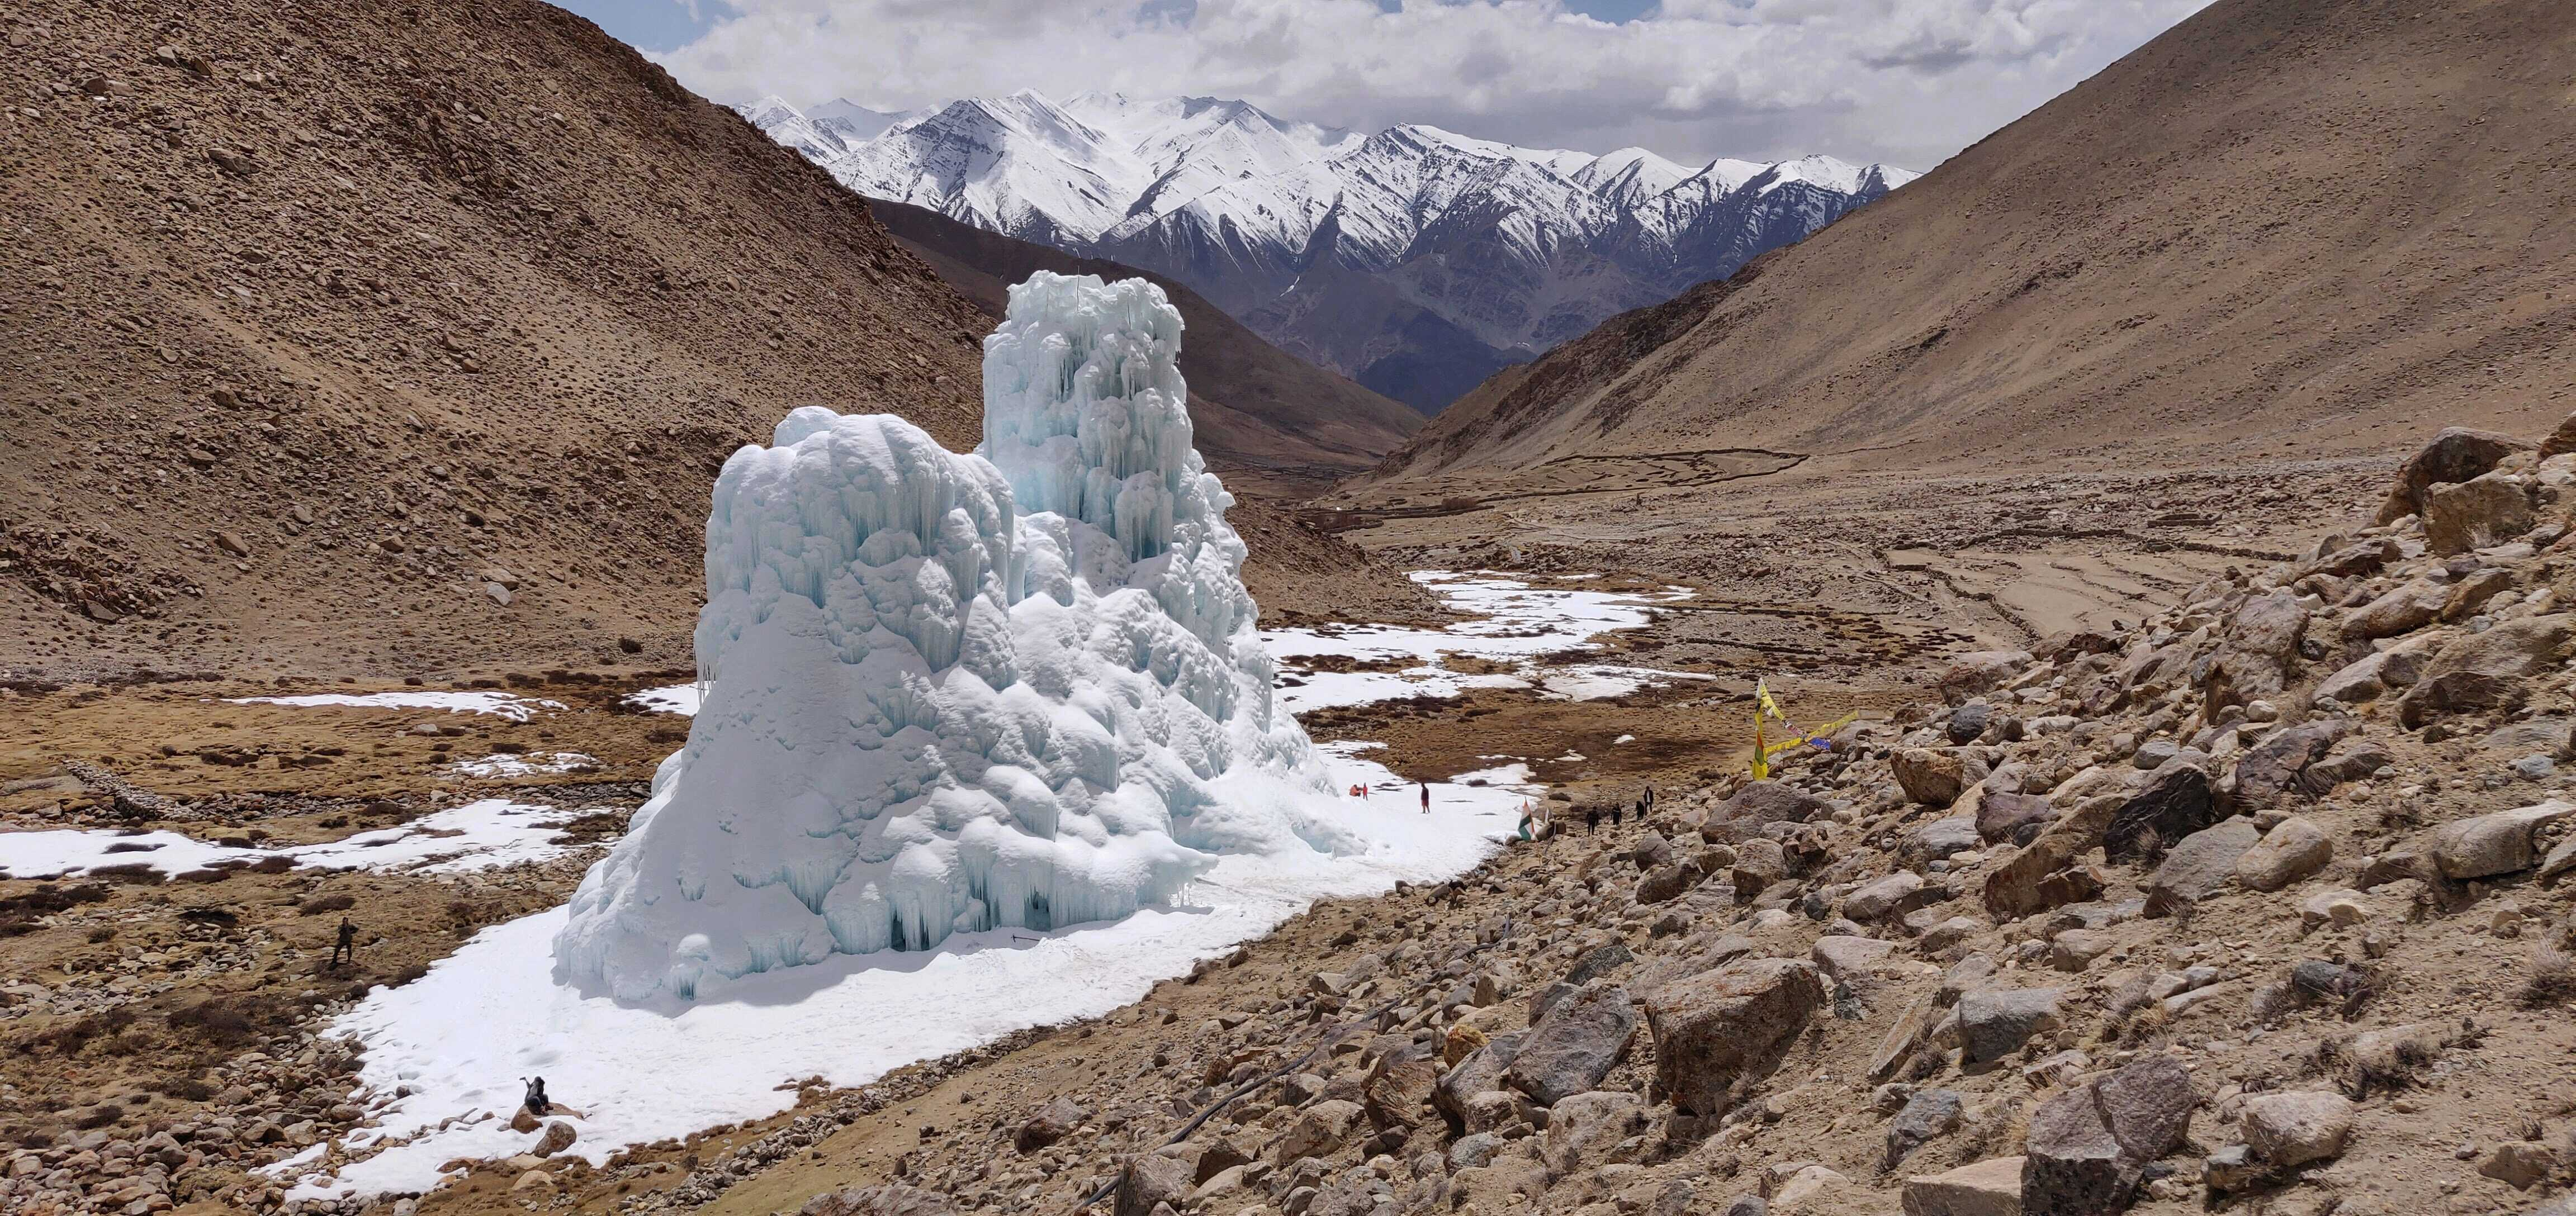
\includegraphics[width=\textwidth]{figs/PIR_example.jpg}

  \caption{Icestupa at Shara, Ladakh, built by local farmers in the winter of 2019-20, survived a full summer melt season and released
  around 8 million litres of water.} 

\label{fig:PIR} 
\end{figure}

\begin{figure}[htb]
  \centering
	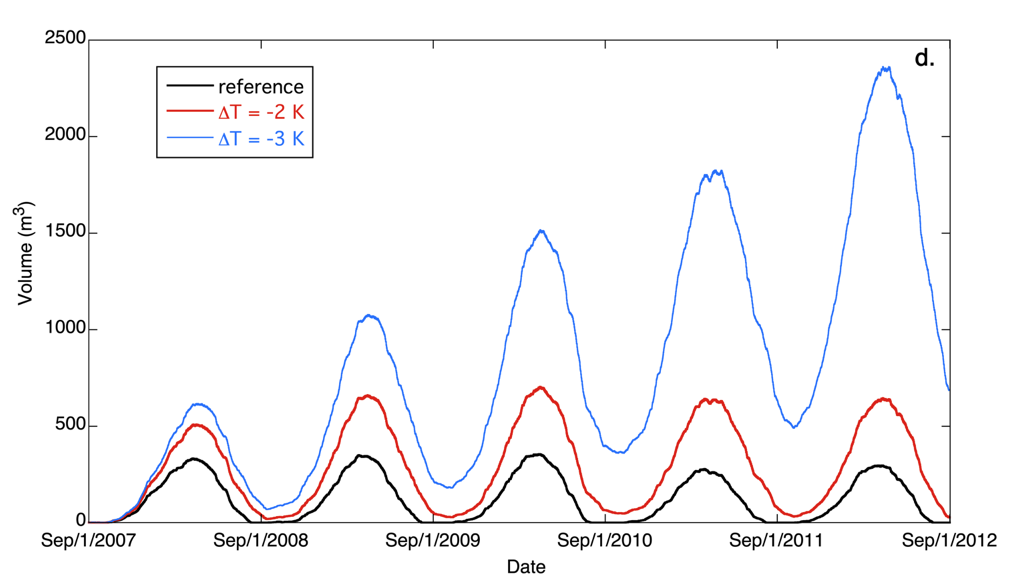
\includegraphics[width=\textwidth]{figs/PIR_evolution.png}
  \caption{The effect of a negative temperature perturbation. For $\Delta T = -3 \degree C$ the icestupa does
  not disappear anymore but is growing from year to year.}
\label{fig:PIR_evolution}
\end{figure}



\subsection{Interannual scale}
\label{sec:interannual}

\begin{figure}[htb]
\centering
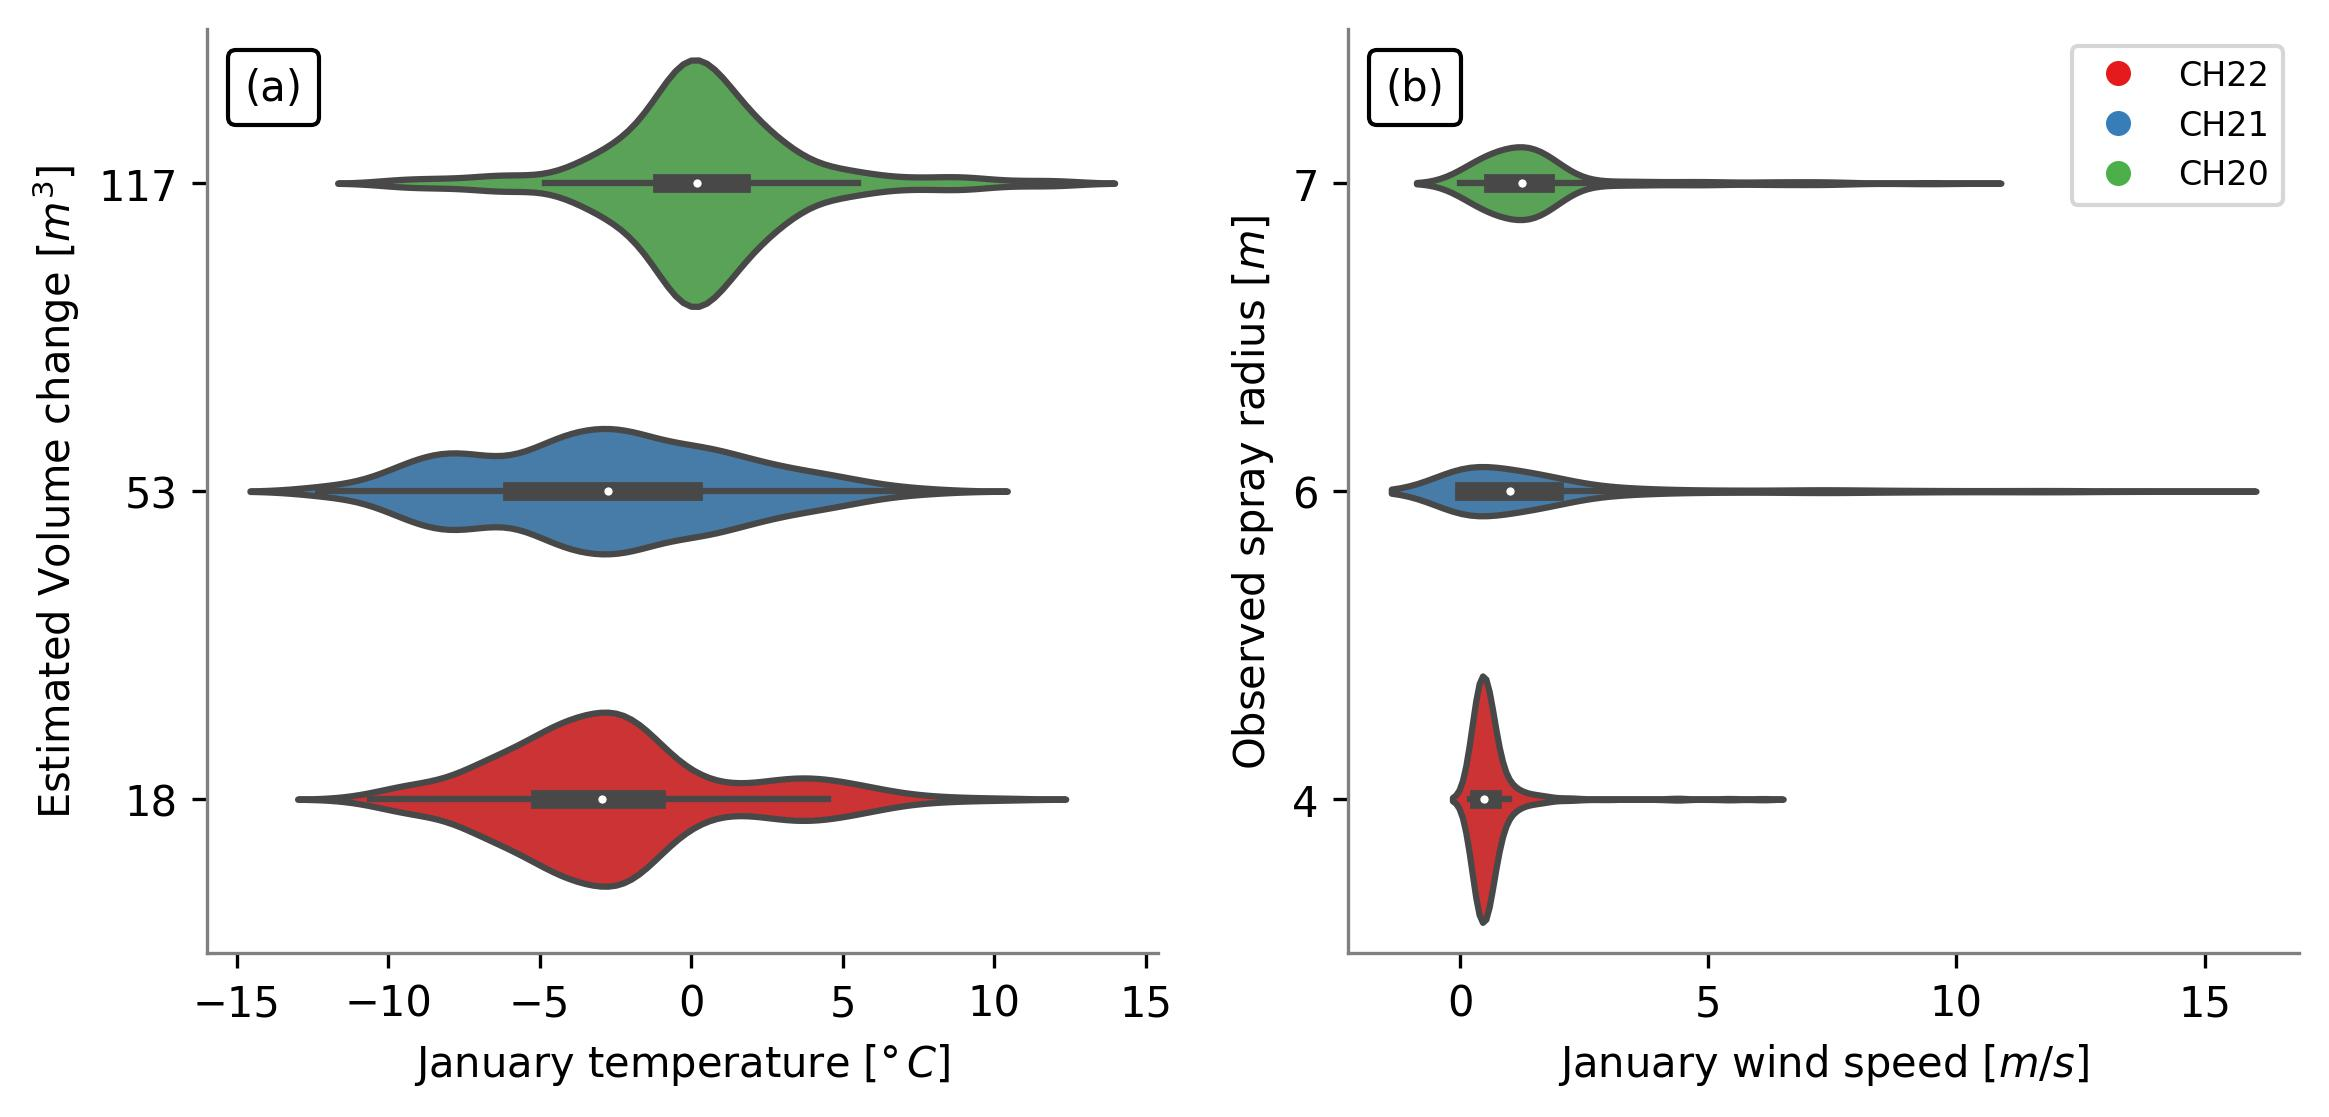
\includegraphics[width=\textwidth]{figs/CH_diffs.jpg}
\caption{(a) Estimated volume change and temperature and (b) Observed spray radius and wind speed
during January for AIRs built across three winters. } 
\label{fig:CH_diffs}
\end{figure}

AIRs built in Switzerland across three winters (CH20, CH21 and CH22) show a decreasing trend in their ice volume
changes for the month of January. Contrary to expectations, this decreasing trend was not caused by increasing
temperatures but rather by decreasing wind speeds (Fig. \ref{fig:CH_diffs}). A process-based analysis revealed
that wind driven redistribution could explain these differences (paper II). The influence of this process on
the fountain spray radius managed to generate AIRs six times bigger in spite of temperatures being 3 $\degree C$
warmer (Fig. \ref{fig:CH_diffs} (b)). 



\section{Metrics to judge site suitability}

Accordingly, we propose two sets of guidelines to identify future construction sites at a regional and a local
scale. These decisions are guided by both the different case studies presented in this thesis and my field
experiences in Ladakh over the past six winters.

\subsection{Regional scale}

\begin{enumerate}

  \item Minimum median monthly temperature less than $0 \degree C$. 
  \item Water supply with median discharge rate more than $2\, l/min$.
  \item Terrain slope between water source and site greater than 20 m every km. 

\end{enumerate}

\subsection{Local scale}

Given a valley or a region satisfying the above requirements, further selection of sites around the particular
water supply can be performed using the criterions below: 

\begin{enumerate}
  \item Water source temperature is higher.
  \item Daylight hours are lower due to shadows.
  \item Altitude is higher.
\end{enumerate}

